\subsection*{Actividad 1.D}
\textbf{Consigna. }
Una inecuación es una desigualdad entre dos expresiones algebraicas,
con una o varias incógnitas.
Los coeficientes de la x también pueden pasar al otro lado como en
las ecuaciones, pero tenemos que cambiar el signo de
desigualdad si el número es negativo.
¿Por qué?

Dados dos números $a, b \in \mathbb{R}$,
tal que \(0 < a < b\),
pordemos concluir que la siguiente inecuación es verdadera:

\begin{align*}
	a < b
\end{align*}

Esto significa que,
en la recta real, \(a\) está a la izquierda de \(b\).
Sin embargo,
si multiplicamos ambos lados por \(-1\),
sin cambiar el sentido de la desigualdad, obtenemos:

\begin{align*}
	-a < -b
\end{align*}

Notar que,
representados en la recta real:

\begin{center}
	\vspace{15pt}
	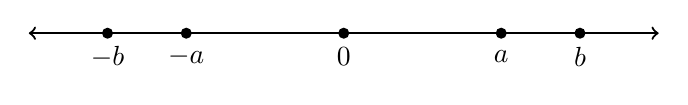
\begin{tikzpicture}
		% Dibuja la recta
		\draw [thick, <->] (-4,0) -- (4,0);

		% Marca los puntos
		\foreach \x in {-3, -2, 0, 2, 3} {
				\fill (\x,0) circle (2pt);
			}

		% Etiquetas
		\node at (-3, -.3) {$-b$};
		\node at (-2, -.3) {$-a$};
		\node at (0, -.3) {$0$};
		\node at (2, -.3) {$a$};
		\node at (3, -.3) {$b$};
	\end{tikzpicture}
	\vspace{15pt}
\end{center}

Por lo cual, \(-a < -b\) es una contradicción.
Con ello, demostramos que,
cuando se opere un producto negativo a ambos lados de una inecuación,
debemos cambiar el sentido de la misma.
